\documentclass[a4paper, 11pt]{article}
\usepackage[utf8]{inputenc}
\usepackage{graphicx} %for figures and pictures
\usepackage[noend]{algorithm2e}
\usepackage{float}
\usepackage{amsmath}
\usepackage{amssymb}
\usepackage{epsfig,floatflt}
\usepackage{physics}
\usepackage[english]{babel}
\usepackage{booktabs}
\usepackage{pgfplotstable,filecontents} %for importing csv as table
%\usepackage{csvsimple} %importing csv as table
\usepackage[round]{natbib}
%\usepackage{cite}
\usepackage[format=plain,
font=it]{caption}
\usepackage{url}
\usepackage{hyperref}
\usepackage{color}
\definecolor{darkred}{rgb}{0.5,0,0}
\definecolor{darkgreen}{rgb}{0,0.5,0}
\definecolor{darkblue}{rgb}{0,0,0.5}

\usepackage{graphicx}
\usepackage{lingmacros}
\usepackage{blindtext}
\usepackage{tree-dvips}
\usepackage{amsmath}
\usepackage{multicol}
\usepackage{mathtools}
\usepackage{hyperref}
\usepackage{graphicx}
\usepackage{amssymb}
\usepackage[table]{xcolor}
\usepackage{textcomp}
\usepackage{subfig} %for dual figures
%\usepackage{floatrow}
%\usepackage{romannum} %for roman numbers
\graphicspath{ {./Latex/} }


\hypersetup{ colorlinks,
	linkcolor=darkblue,
	filecolor=darkgreen,
	urlcolor=darkred,
	citecolor=darkblue }

\graphicspath{{../figures/}}
\DeclareGraphicsExtensions{.pdf}

\begin{document}

\begin{titlepage}
    \begin{center}
        \vspace*{1cm}
            
        \Huge
        \textbf{Model-based IDF-curves in Norway}
            
        \vspace{0.5cm}
        \LARGE
        Can IDF-curves be produced based on AROME model output?
            
        \vspace{1.5cm}
            
        \textbf{Eirik Nordgård}
            
        \vfill
        
\includegraphics[width=0.4\textwidth]{figures/uio_logo.png}
            
        A thesis presented for the degree of\\
        Master of Meteorology
            
        \vspace{0.8cm}
            
        
\includegraphics[width=0.4\textwidth]{figures/uio.png}
            
        \Large
        Department of Geosciences\\
        University of Oslo\\
        Norway\\
        June 2021
            
    \end{center}
\end{titlepage}

\tableofcontents

%\section{Abstract}
%\label{sec:abstract}

\thispagestyle{plain}
\begin{center}
    \Large
    \textbf{Thesis Title}
        
    \vspace{0.4cm}
    \large
    Thesis Subtitle
        
    \vspace{0.4cm}
    \textbf{Author Name}
       
    \vspace{0.9cm}
    \textbf{Abstract}
\end{center}

\section{Introduction}
\label{sec:introduction}
\subsection{Introduction}
Introduction here 

From meeting:
Assumption: climate is stationary.
Do not focus on wrong or wright with the 9g vs 1g model. All the methods are alternatives. Discuss how you did it with the models and how to interepret the results they give. Use the word "concistency" rather than right or wrong. One version of the model may be more consistent with the station based idf values than others.
Try to aim for: wuantifieng change in percent from 1g to the various 9g methods. Discuss the change of results based on method.
Also include 9g indivdual rom a couple of stations to highlight the individual station uncertanty (topography play an inportant role in small scale conventve evetns). Discuss and cuantify uncertanty. 
Inclue sruface scheme (one paragraph) in the AROME descripton.
Discuss the method with ANita, and then Jana for input. 

\subsection{Research aim?}
Firstly the main goal for this thesis was to investigate how future IDF values differ from values obtained by historic station data. The idea was to verify the general opinion on increased precipitation extremes through the IDF curved derived by modelled data. One step towards this goal is to verify whether the modelled precipitation can at all be used for this purpose. To check this, I must first evaluate the IDF-values against some stations. Along the way I must define what return periods are realistically represented by the data. If they match I can proceed to do an analysis of other locations. If not I should investigate why, or to what extent these data can be used in terms of IDF values in Norway.

\\
For an introduction: get inspiration in text from orskar and lind about model-setup of HARMONIE: \cite{lind_arome} 

\\
A high-resolution forecast model like AROME are overall better in capturing precipitation magnitude and location compared to coarser-resolution models. In MÜller et al. 2017 \cite{muller} they performed a case-study comparing precipitation events forecasted by AROME to the coarser-resolution ECMWF-IFS model. \textbf{not sure if this is relevant, but as an introduction it will do for now.. maybe this could be part of an introduction in stead?}  

\section{Background}
\label{sec:background}

\subsection{Meteorological Background}

Explain convention and what generally causes the most extreme precipitation on the different durations. Present some typical precipitation values at the selected durations values?

Maybe the GEO4902 work can be included here in the background? Or it can be included as a separate section to highlight problems with forecasting extreme events? This can also be used to justify why we have to choose the maximum values from multiple grid.boxes around the respective station.   
one paper under AROME folder also highlights what effect horizontal resolution have on extreme precipitation. 

\subsection{Area}

The area investigated in this thesis is Oslo, the capitol of Norway. This location is selected for a number of reasons. Firstly there are multiple stations in the area witch have long, high quality data series of precipitation. This is essential because it allows for comparison to the modeled IDF values. When analysing IDF curves short time series is a problem in it self, therefore having multiple high quality data series is very valuable to the analysis. Also, multiple stations covering a rather small area like in this case may highlight certain features in the IDF curves related to topography or other mechanisms influencing precipitation that would otherwise have been hidden. Secondly the Oslo area is a typical urban area, making it vulnerable to short duration extreme precipitation. Improving the knowledge on extreme precipitation events may potentially save the area and its population for large weather-related costs in the future. Another reason for selecting this area was the availability of cleaned data. Data from the selected stations had been cleaned and checked for analysis beforehand as part of the \textbf{Julia paper (how do I address this?)}. 

\subsection{Data}
\subsubsection{Measurements}
Precipitation measurements used in this project is obtained from pluviometers operated by the Norwegian Water Resources and Energy Directorate (NVE) or the respective municipalities in corporation with  MET Norway. Since the late 1990s and early 2000s the operating pluviometer has been the Lambrecht 1518H3 tipping bucket pluviometer manufactured by the German company Lambrecht meteo GmbH \cite{lutz_idf}. The Lambrecht pluviometer has a measuring range of 0.1 mm precipitation at time resolution of 1 minute and a given accuracy of $\pm$ 2$\%$. Intensity correction is done to account for loss of rain due to the time required for the bucket to tip. MET Norway supervised the installation of the pluviometers and ensured installation according to the recommendations from the World Meteorological Organization (WMO). Additionally MET Norway performed quality control and storage on all data from the pluviometers. Before the now operational Lambrecht some of the stations operated with the Norwegian produced pluviograph Plumatic, manufactured by Kongsberg Våpenfabrikk A/S. It was replaced partially due to is lack of heating, making it operational only in the extended summer months, from mid-April to mid-October. The Lambrecht also suffers from poorer data quality during winter due to snowcaps or ice-slush obstruction spite been heated.  

The proposed method in this study requires annual maxima for each duration as input, thus a requirement for season completeness is necessary. The requirement where here set to at least 80\% of the days throughout the season covered and of good quality. Hence the precipitation series extracted where shorter than the total operational period for all stations. The number of extracted years with annual maxima is found in Table \textbf{number of table below}. Lutz et al 2020 analysed monthly precipitation for 1,2 and 3 hours in two locations in Oslo and found that the highest occurrence of short-duration, high-intensity precipitation was during the summer months. In combination with lack of high-quality data during the winter period, especially from before the 1990s when the Plumatic pluviometer were still in use, makes the extended summer period, 1st of May to 30th of September, best suited for the IDF analysis in this study. Furthermore, time series of 10 years is here considered to be an absolute minimum for calculation of IDF values. The twelve stations listed in Table \textbf{table under, need numer} are the ones left meeting these criteria in the municipality of Oslo.   

\\

\begin{center}
\begin{tabular}{ |p{3cm}||p{3cm}|p{3cm}|p{3cm}|  }
\hline
\multicolumn{4}{|c|}{Oslo Stations} \\
\hline
 Station Name & Station NR & Years AM & Operational From\\
 Ljabruveien & 17980  & 17 &  01.01.1985-\\
 Lambergseter & 18020 & 25 & 15.05.1999-\\
 Hovin & 18210 & 17 & 15.01.1999-\\
 Haugenstua & 18269 & 15 & 01.01.2000-\\
 Vestli & 18270 & 32 & 18.04.1974-\\
 Hausmannsgt & 18320 & 20 & 21.06.1984-04.11.2013\\
 Disen & 18420 & 20 & 02.06.1998-\\
 Vestre Vika & 18640 & 13 & 22.05.1974-03.10.1998\\
 Blindern PLU & 18701 & 48 & 16.04.1968-\\
 Bygdøy & 18815 & 16 & 01.01.2000-\\
 Besserud & 18920 & 13 & 29.09.2998-\\
 Lilleaker & 18980 & 13 & 01.01.2000-   
\end{tabular}
\end{center}

\textbf{the section "measurements" in Lutz et al., 2020 has the description of the station data. Essentially annual maxima for each duration and station.} Tipping bucket pluviometers does not function properly during winter, so this is basically summer-data. Time series of 10 years is concidered an asolute minimum here, hence the choice of these 12 stations (you can also include the two from Bærum if you get the data). 

\subsubsection{AROME model and data}

For this study precipitation output from the non-hydrostatic Applications of Research to Operations at Mesoscale (AROME)\cite{seity_arome} model have been used. The model is developed by Météo-France and is operated by a cooperative effort named Meteorological Cooperation on Operational Numerical Weather Prediction (MetCoOp) between the Norwegian Meteorological Institute (MET-Norway) and the Swedish Meteorological and Hydrological Institute (SMHI). AROME is used operationally for high-resolution numerical weather prediction (NWP) since 2008 and has recently been used in a climate-configuration for long-term climate simulations \cite{lind_arome]}. Being one of the first long-term climate simulations on regional convection-permitting (\<4km) scales for the Fenno-Scandinavian region this data-set provides added opportunities for analysis of extreme precipitation.  
\\
\\
HARMONIE-Climate cycle 38 (HCLIM38) on 3 km resolution with explicit deep convection is the parenting model used in the this study (Lindstedt et al. 2015\cite{lindstedt_hclim}; Lind et al. 2016\cite{lind_hclim}). A comprehensive description of the model system is presented in Belušić et al.(2020)\cite{belusic_hclim}. The model proved strong improvement on representation of precipitation compared to similar model-setups with coarser models in Lind et al. 2020 \cite{lind_arome}. Most evident was the improvement in reduction of "drizzle" and increased occurrence of high intensity precipitation events in addition to better timing and amplitude of the diurnal cycle. The simulations was conducted within the Nordic Convection Permetting Climate Projections project (NorCP), which is one of the leading projects on increasing knowledge of climate changes and processes over the Fenno-Scandinavian region. Here the model-run with the AROME physics package is applied. AROME (Bengtsson et al. 2017)\cite{bengtsson_arome} is designed for convection-permitting scales and non-hydrostatic dynamics with 65 vertical layers. The boundary state for HCLIM38-AROME (HCLIM3) is obtained from the global ERA-Interim reanalysis (Berrisford et al. 2011)\cite{erai}. This data has a horizontal grid of approximately 80 km, available every 6 hour. An alternative set of boundary data from EC-Earth (ECE) is also applied, providing a slightly different climate simulation.    
ECE
\\
HCLIM3
surface and precip representation

\cite{lind_arome} citation figure arome domain 
\begin{figure}
    \centering
    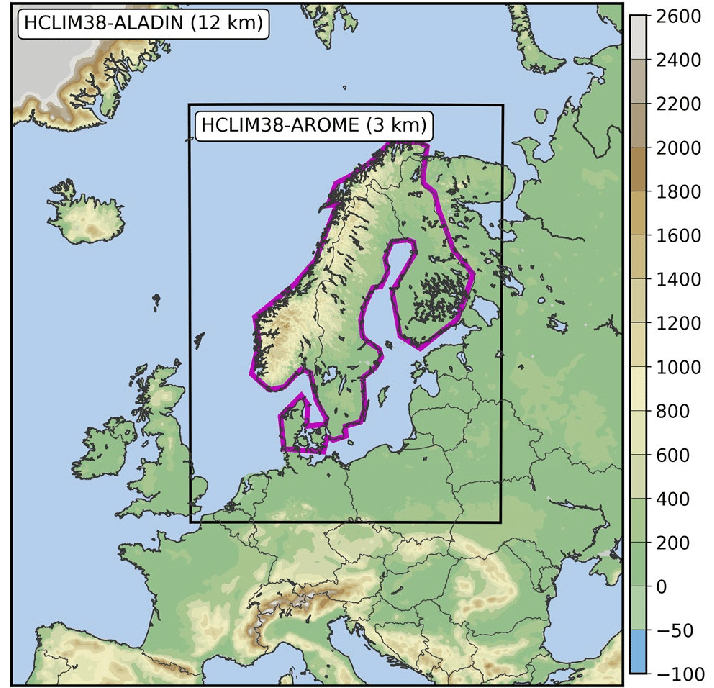
\includegraphics[scale=0.4]{figures/arome_domain.png}
    \caption{Domain used for HCLIM38-ALADIN (12km) simulation and domain used for HCLIM38-AROME (3km) simulation in the inner black rectangle. The colorscale represents the altitude above mean sea level in meters, and the magent colored area defines the Fenno-Scandinavian region. Source: Lind et al. 2020 \cite{lind_arome}}
    \label{fig:arome_domain}
\end{figure}

\subsubsection{AROME performance: an example}
Maybe an example showing how AROME have performed well on small-scale events and another on where it have performed poorly? 



\section{Theory and method}
\label{sec:theory}

\section{Method}
\subsection{You should clarify these things:}

\begin{itemize}
\item The GEV framework 
\item The Bayesian framework, highlight probabilistic aspect and advantages (and disadvantages)
\item Some description/justification of the chosen return levels and duration
\item Describe the station data from MET. Describe the modelled data from AROME. 
\item If there are any other aspects of the code you should include this as well.
\item maybe a short paragraph on the choice/restriction on the shape parameter. 
\item Later: describe how the performance of the historic modelled vs. measurement-based curves are evaluated. 
\end{itemize}

Clarify with Malte how to refer to Julia and Anitaz study. My study is after all (to a degree) based on their method, and this should be highlighted somewhere and probably in a certain way?

\subsection{The General Idea of IDF values} 


Intensity-Duration-Frequency (IDF) curves comprise an estimate of rainfall intensities of different durations and recurrence intervals. Durations commonly range from minutes to days and recurrence intervals often range from a year to a couple hundreds of years. \textbf{insert example of IDF values for a given duration and return period as illustration}. The curves can either be calculated for a large region or for a single point. Depending on the topography and governing precipitation processes and patterns the IDF values may differ quite a lot between locations only kilometres apart. \textit{Duration} refers to the length of the precipitation event. Maximum rainfall intensity for each duration can be related to corresponding\textit{recurrence intervals} or \textit{return periods}. The return period is defined as $T = 1/P$ where $P$ is the annual exceedance probability. $P = 0.1$  (10\%)  implies that a precipitation event of a certain magnitude has a return period $T$ of ten years. It can also be interpreted as a 10\% chance of exceeding the given magnitude in any year. \textbf{this is just my understanding.find a source on this?}. (https://web.arch.virginia.edu/struct/arch721/content/lectures/lec-06/page-2.html) Thus, the higher return period $T$ of an event, the less likely it is that this event will occur during a given year. \textbf{possibly elaborate on this from the previous link}. The corresponding cumulative Distribution Frequency (CDF) $F$ will be: $F = 1-P = 1-1/T$. Once $F$ is known the maximum rainfall intensity for each duration and return period is determined through the chosen PDF (e.g GEV, Pearson type \textbf{3 in roman} distributions, Gumbel) (Nhat et al., 2006). IDF curves can then be presented as precipitation from one duration at all return periods and as precipitation at one return period on all durations. 


\subsection{IDF calculation packages}

R software and packages on extreme value statistics has been used to perform the IDF calculations (R Core Team, 2013). R is a language and environment for statistical computing and graphics, and the R software is available as Free Software under the terms of the Free Software Foundation's GNU General Public License (https://www.r-project.org/about.html). Functionalities in the R package \textit{extRemes}, Weather and Climate Applications of Extreme Value Analysis, have been used for an extreme value analysis. The package allows for parameter-estimation on extreme-value distributions, implementation of different inference methods and more(extRemes by Gilleland, 2020). The function \textit{fevd} with arguments \textit{type=GEV} and \textit{method=Bayesian} fits the univariate general extreme value distribution to the precipitation data(RDocumentation, fevd). The type-argument states which extreme value distribution to fit to data, while the method-argument states which type of estimation method should be used. The fit is done for desired quantiles and return levels for all durations is calculated.  

 

\subsection{Practices in Computation of IDF values}

Short-duration precipitation statistics is often presented with Intensity-Duration-Frequency (IDF) curves. IDF curves provide information on duration and frequency of pre-defined precipitation events, and they are often used in planning and design of infrastructure and other water-managing structures. There are many ways to calculate IDF values, thus different methods are used in different countries. In Sweden two of these have been applied when Olsson et al. (2019) fitted the Generalized Extreme Values (GEV) distribution to block maxima and the Generalized Pareto distribution to Peak-Over-Threshold events (Hosking et al., 1987) to calculate regional short-duration rainfall. In Québec in Canada was a Bayesian approach with standard parameter estimation for the GEV distribution used (Huard et al., 2010). In this study the Bayesian approach was recommended for further studies as it implicitly include an estimation of the uncertainty of the IDF values. Mohymont et al. (2004) used a GEV distribution and a Gumbel distribution to establish IDF-curves for the tropical Central Africa. The most recent methodology for estimating IDF values in Norway is based on fitting a Gumbel distribution to the N-highest measurements (N being the time-series length in years). Lutz et al. (2020) explored ways to update the Norwegian IDF routine, fitting a General Extreme Value (GEV) distribution for annual maximum precipitation using a modified Maximum Likelihood estimation and a Bayesian inference. Here the Bayesian method performed best in two goodness-of-fit tests and thus was recommended for IDF estimation for Oslo in Norway.

One profound challenge in estimating IDF values for extreme precipitation is the availability of data. Short data series yields very large uncertainties in precipitation magnitude for large return periods. To properly analyse IDF curves and the potential impacts of the events they describe it is crucial to capture and understand the uncertainties of the curves. As recommended in Huard et al. (2010) and practised in Lutz et al. (2020) fitting an GEV distribution using a Bayesian method will be applied in this study for best estimates of the IDF values and well-described uncertainty.  
 

\subsection{GEV distribution and extreme value statistics}

Extreme value theory provides the statistical framework needed to infer probability of very rare or extreme events. The Generalized Extreme Value distribution describes a family of three possible types of distributions of block maxima of a given variable, allowing a continuous range of possible distribution shapes. These distributions are called Type 1, Type 2 or Type 3, also known as Gumbel, Fréchet and Weibull respectively. The block maxima distribution converges to a GEV, G(x), distribution once the record length approaches infinity. Being a three-parameter distribution, G(x) can be written on the form:

\begin{equation}
	G(x) = exp\bigg\{-\left[1+\zeta(\frac{x-\mu}{\sigma})\right]^\frac{-1}{\zeta}\bigg\}
	\label{eq:gev}
\end{equation}

for 
\begin{equation}
	1+\zeta(\frac{x-\mu}{\sigma} \textgreater 0
\end{equation}

where $\mu$ is location, $\sigma$ is scale and $\zeta$ is shape (Dyrrdal et al., 2015). Since the extremes are determined from the tail of the distribution, they are heavily affected by the choice of $\zeta$. $\zeta$ determines whether the distribution converges towards Gumbel ($\zeta$=0) with a light upper tail, Fréchet ($\zeta$\textgreater0) with a heavy upper tail or Weibull ($\zeta$\textless0) which is bounded from above (Dyrrdal et al., 2014). As the shape parameter describes the tail of the distribution it will severely affect the estimates for long return periods. The shape parameter can be both positive and negative, depending on the location of interest. Poor choice of this parameter may provide unrealistic precipitation estimates, especially on the longer return periods, thus Lutz et al. (2020) introduced a prior distribution to constrain the $\zeta$ parameter of the GEV distribution.\textbf{(or should I refer to the paper she is referring to (the original source)?.}. Maybe include some more information on on the parameters? 

\subsection{Bayesian Approach}
\subsubsection{Basics}
In general the goal is to estimate parameters of a distribution to best fit data. Given a generic parameter $\beta$, the likelihood function is the probability density of the observed data as a function of $\beta$. $\beta$s with high likelihood correspond to models which give high probability to the observed data. Traditionally, a maximum likelihood estimation seeks to adopt the model with greatest likelihood, namely the model that assigns the highest probability to the observed data. Bayesian inference provide an alternative method to draw inference from a likelihood function (http://www.mas.ncl.ac.uk/~nlf8/shortcourse/part5.pdf many things are well formulated in this pdf, but I havent found its origin yet). 

Here a Bayesian inference is used to estimate one probability distribution for the parameter set $\sigma$ containing the three GEV parameters, $\alpha = (\sigma, \zeta, \mu)$. These parameters are treated as random variables with prior distributions, distributions of the parameter prior to the inclusion of data $x = (x_1, x_2,...,x_n)$. Bayes` Theorem (need source?) states that the probability of an event is dependent on prior knowledge of conditions that are relevant to the event. The theorem states:

\begin{equation}
P(\alpha \vert x) = \frac{L(x \vert \alpha)P(\alpha)}{P(x)},
\label{bays}
\end{equation}

where $P(\alpha \vert x)$ is the probability density function of $\alpha$ given the observations $x$. $L(x \vert \alpha)$ is the likelihood function an $P(\alpha)$ is the GEV parameters (prior probability of $\alpha$, better to use this instead of "GEV parameters"?). Since $P(x)$ is constant Equation \eqref{bays} can be written as 

\begin{equation}
P(\alpha \vert x)\propto L(x \vert \alpha)P(\alpha)
\end{equation}  
or
\begin{equation}
posterior \propto prior * likelihood
\end{equation}
where the $posterior$ is the distribution of $\alpha$ after the inclusion of data. As done in Lutz et al. (2020) $P(\alpha \vert x)$ is sampled using the Markov Chain Monte Carlo (MCMC) method with 50,000 iterations, where the last 3000 is used to have stability in the simulated parameters. \textbf{maybe include some background in MCMC as well?}. Furthermore, the posterior distribution allows for direct derivation of quantiles. Here the 95\% credible interval is used. 


\subsubsection{Advantages}
Choosing a Bayesian analysis of extremes over a more traditional likelihood approach can have various advantages. Incorporating other sources of information, like a prior distribution, to the analysis is considered a large advantage given the scarce nature of the extremes. Making good use of any knowledge on the distribution Another major advantage is that the variance of the posterior distribution can be used can be used to calculate the precision of the inference. This way the resulting IDF values can be presented with desired confidence levels.   

%http://www.mas.ncl.ac.uk/~nlf8/shortcourse/part5.pdf

%https://www.researchgate.net/publication/226610355_A_full_Bayesian_approach_to_generalized_maximum_likelihood_estimation_of_generalized_extreme_value_distribution


\subsection{Application of GEV distribution}
By fitting a sample of extremes to the GEV distribution we can obtain the parameters that best explains the probability distribution of those extremes. We can estimate how often the extreme quantiles occur with a certain return level from the fitted distribution. One example is how large a precipitation event can be expected to be with a return period of 100 years. This values is expected to be equalled or exceeded on average once during this return period \cite{gmao}.

\subsection{Weakness of GEV statistics}

here the length of the time series mattters, the topography of the selected area, the spred of the data it self. Many thing will affect the resultingIDF values. 

\section{Issues}
\label{sec:issues}

\subsubsection{Issues with time series length}

As with any other extreme value problem, the data series length have a major impact on the resulting statistics. The problem arises when a time series of a given length is used to infer statistics for return periods far longer than the time series itself. Given a time series of ten years, it is unlikely that a maximum value for a return period of 100 years is captured in that time series. The issue of what return periods could be represented by your data series depends a lot on what type of phenomena you are describing. In this case we are concerned with precipitation, and there are some limits to how large and rare an event could be. A time series of 10-15 years could probably represent a return period of 20-40, while a time series of 100 years could probably represent a return period of 500 years or more. 

Anther issue arising when using short time series in this analysis is the possibility of getting decreasing IDF-values for increasing duration. Each duration is fitted individually. Since the resulting IDF-curve is an fit to the available years, some large or low values in a short time series will have a greater impact on the curve than the same values in a longer time series. This means that some large return values for a given duration may affect the curve more than normal return values for another longer duration. Thus, as a result of using a short time series, it is possible to experience decreasing return values for increasing duration in some cases. That being said, this is a purely statistical phenomena. The true maxima of a precipitation event will always increase with duration.    


\subsubsection{Possible roadblock in extreme value theory}
To perform extreme values statistics ideally you would benefit from having a long time series. The longer the time series, the higher probability that an extreme event for a given return period would have happened. Using a time series of 10-20 years has a low probability of containing a 1-in-200 year event. Where this given time series data of 400 years, the probability of it containing the 1-in-200 year event would drastically increase. Since most of the data provided are on length 15-35 years it is highly questionable if they can at all represent return periods of longer than 20-30 years. 


\subsection{note}
Traditionally IDF-values are calculated based on measured data from available stations. Moving towards IDF-curves based on modelled data it is necessary to investigate whether the modelled data captures the precipitation extremes at the given locations. The IDF-analysis will be of little interest if the analyses it self does not reflect true nature as captured by the stations. However, should the modelled data fail to capture the extremes it is an interesting study to find out why this might be the case.   

\subsection{How is the model built}

\section{Results}
\label{sec:results}

\subsection{Preliminary findings}

To find the best model-fit to the station data for the historical period a 9-point grid around the grid closest to the station is used. The maximum precipitation value for each time step is chosen out of the 9 grid points. This is done to minimize the risk of missing an modelled event next to the station grid-point. An event modelled at a certain grid-point might as well happen at the grid-point next to it. To evaluate if this grid selection is better than choosing the grid-point closest to the stations the absolute average difference between the station values and the model values for all durations is calculated for both the 1 grid-procedure and the 9-grid-procedure. If the difference is 0 it means the modelled values are equal to the station-values.  

\begin{table}
\begin{tabular}{ c c c c }

Duration & 1grid & 9grid & diff 1g-9g \\
2 & 2.93 & 8.22 & -5.30 \\
5 & 5.62 & 8.54 & -2.92 \\
10 & 7.86 & 8.93 & -1.07 \\
20 & 10.23 & 9.66 & 0.57 \\
25 & 11.04 & 9.96 & 1.08 \\
50 & 13.71 & 11.19 & 2.52 \\
100 & 16.68 & 12.73 & 3.95 \\
200 & 20.02 & 14.58 & 5.44
\end{tabular}
    \label{grid}
\end{tabular}
\caption{Grid selection. Positive difference: 9grid is better. Negative: 1grid is better}
\end{table}

As displayed is Table \ref{grid} the 9grid-selection outperforms the regular 1grid-selection on the larger return periods, while it is the opposite for smaller return periods.
\textbf{Whys is this the case?}

\subsection{Surrounding grid points Blindern station}

It turned out that the "1grid" approach underestimated the returnvalues, while the "9grid" approach overestimated them. I have calculated the mean difference between the station Blindern and the individual gridpoints surrounding the station to check if any of the gridpoints have particular large impact on the maximum value chosen per time step in the "9g" analysis. The gridpoint to the south and south-west where further away from the station than the other directions by a huge margin. For some return periods the difference where more than twice as large as the smallest differnece for that return period. These directions may affect the overall "9grid" method too much.   

In the "retlev" values in "IDF ECE Blindern 9grid.csv" is smaller for almost all directions and return periods. This is a mismatch with the resulting figures from the 9grid selection method. For all return periods in these figure the Blindrn return values are alot higher for the modeled data over the station data. So why are all return values from the grid points around blindern lower than the station? something is incorrect.

The individual 9g grid points have very lov mean return values for all return periods compared to the first 9g method. Should be the same. 

\subsection{9grid mean vs max method}
Previously the selection method was based on choosing the maximum value per time-step out of the nine gridpoints, forming a one-dimensional timeseries. Then the annual maxima was extracted for each duration. This approach was designed to maximize the chance of capturing an extreme event in close proximity to the station. As discussed above (?) this method appears to "optimize" the modeled precipitation and hence overestimate the return values. Retunvalues for all stations and almost all durations are within the 95 percentile of the station-based retunvalues for the larger returnperiods. This is not surprising given the enormous confidence interval in the largest retunperiods at up to around 200 mmm for the largest durations for some stations. For the smaller returnperiods like 2 and 5 years the method is outside the 95 percentile of the station-based returnvalues. Here the confidence interval is of coarse noticeably smaller. \textbf{make sure its even relevant to comapre this against the confidence interval to the stat based values. Justify it somewhere}.  

make a comment on how the 9grid first method follows the large (100 and 200) returnperiods station idf curves very well for the stations with large confidence intervals. Especially Bygdøy and Besserud and partially Haugenstua (for large durations on Haugenstua).

The two "new"/other 9-grid based selection methods are built differently. Now the annual maximum value for each of the nine  gridpoints for each duration is extracted directly and put into a 3x3 matrix. Either maximum ($MAX$) or mean ($MEAN$)values of the nine is then calculated per duration to give a one-dimensional data series. The $MAX$ alternative is designed to be a less aggressive optimisation of the annual maximum values around the station compared to the other nine-grid maximum selection method \textbf{make a name for this one as well!}. The  $MAX$ maximization method is possibly closer to the real world compared to the \textbf{$XXX$} method. Extracting maximum value for each timestep out of the nine gridpoints might be artificial in one way, since the annual maxima for any duration may be composed from different locations. The $MAX$ method is on the other hand more realistic in the sens that the annul maxima for certain year always origins from one gridpoint. 

\textbf{Here (or later) you can discuss what the station is actually representing. It might be that the $XXX$ method is very representative for the area in general. It would be interesting to check how the station-based IDF curves compares to observations. If these curves are underestimating the observations $XXX$ might be very well suited to represent the overall conditions fr extreme precipitation in the area. Also, describing the methods for extraction should be in the methods section, not here in results}

The resulting $MEAN$ method provides very similar returnvalues to the $1GRID$ method for all stations and all durations. For short returnperiods like 2 or 5 years the returnlevels are close to identical to the $1GRID$ method for all durations and stations, while for the larger returnperiods like 100 or 200 years the $MEAN$ method yields slightly smaller returnvalues for durations up to around 3 hours. This difference appears a smoother inclination of returnvalues compares to the very flat evolution of the $1GRID$ returnvalues for durations between 90 minutes and 3 hours. Out of all the methods the $1GRID$ and the $MEAN$ methods are clearly producing the smallest returnlevels for all stations and durations, and they are consequently smaller compared to the station-based values. Both the $MEAN$ and the $1GRID$ have almost identical returnvalues for all durations on short returnperiods for stations 18701 Blindern, 18320 Hausmansgate and 18270 Vestli. 

\begin{figure}[hbt!]
    \centering
    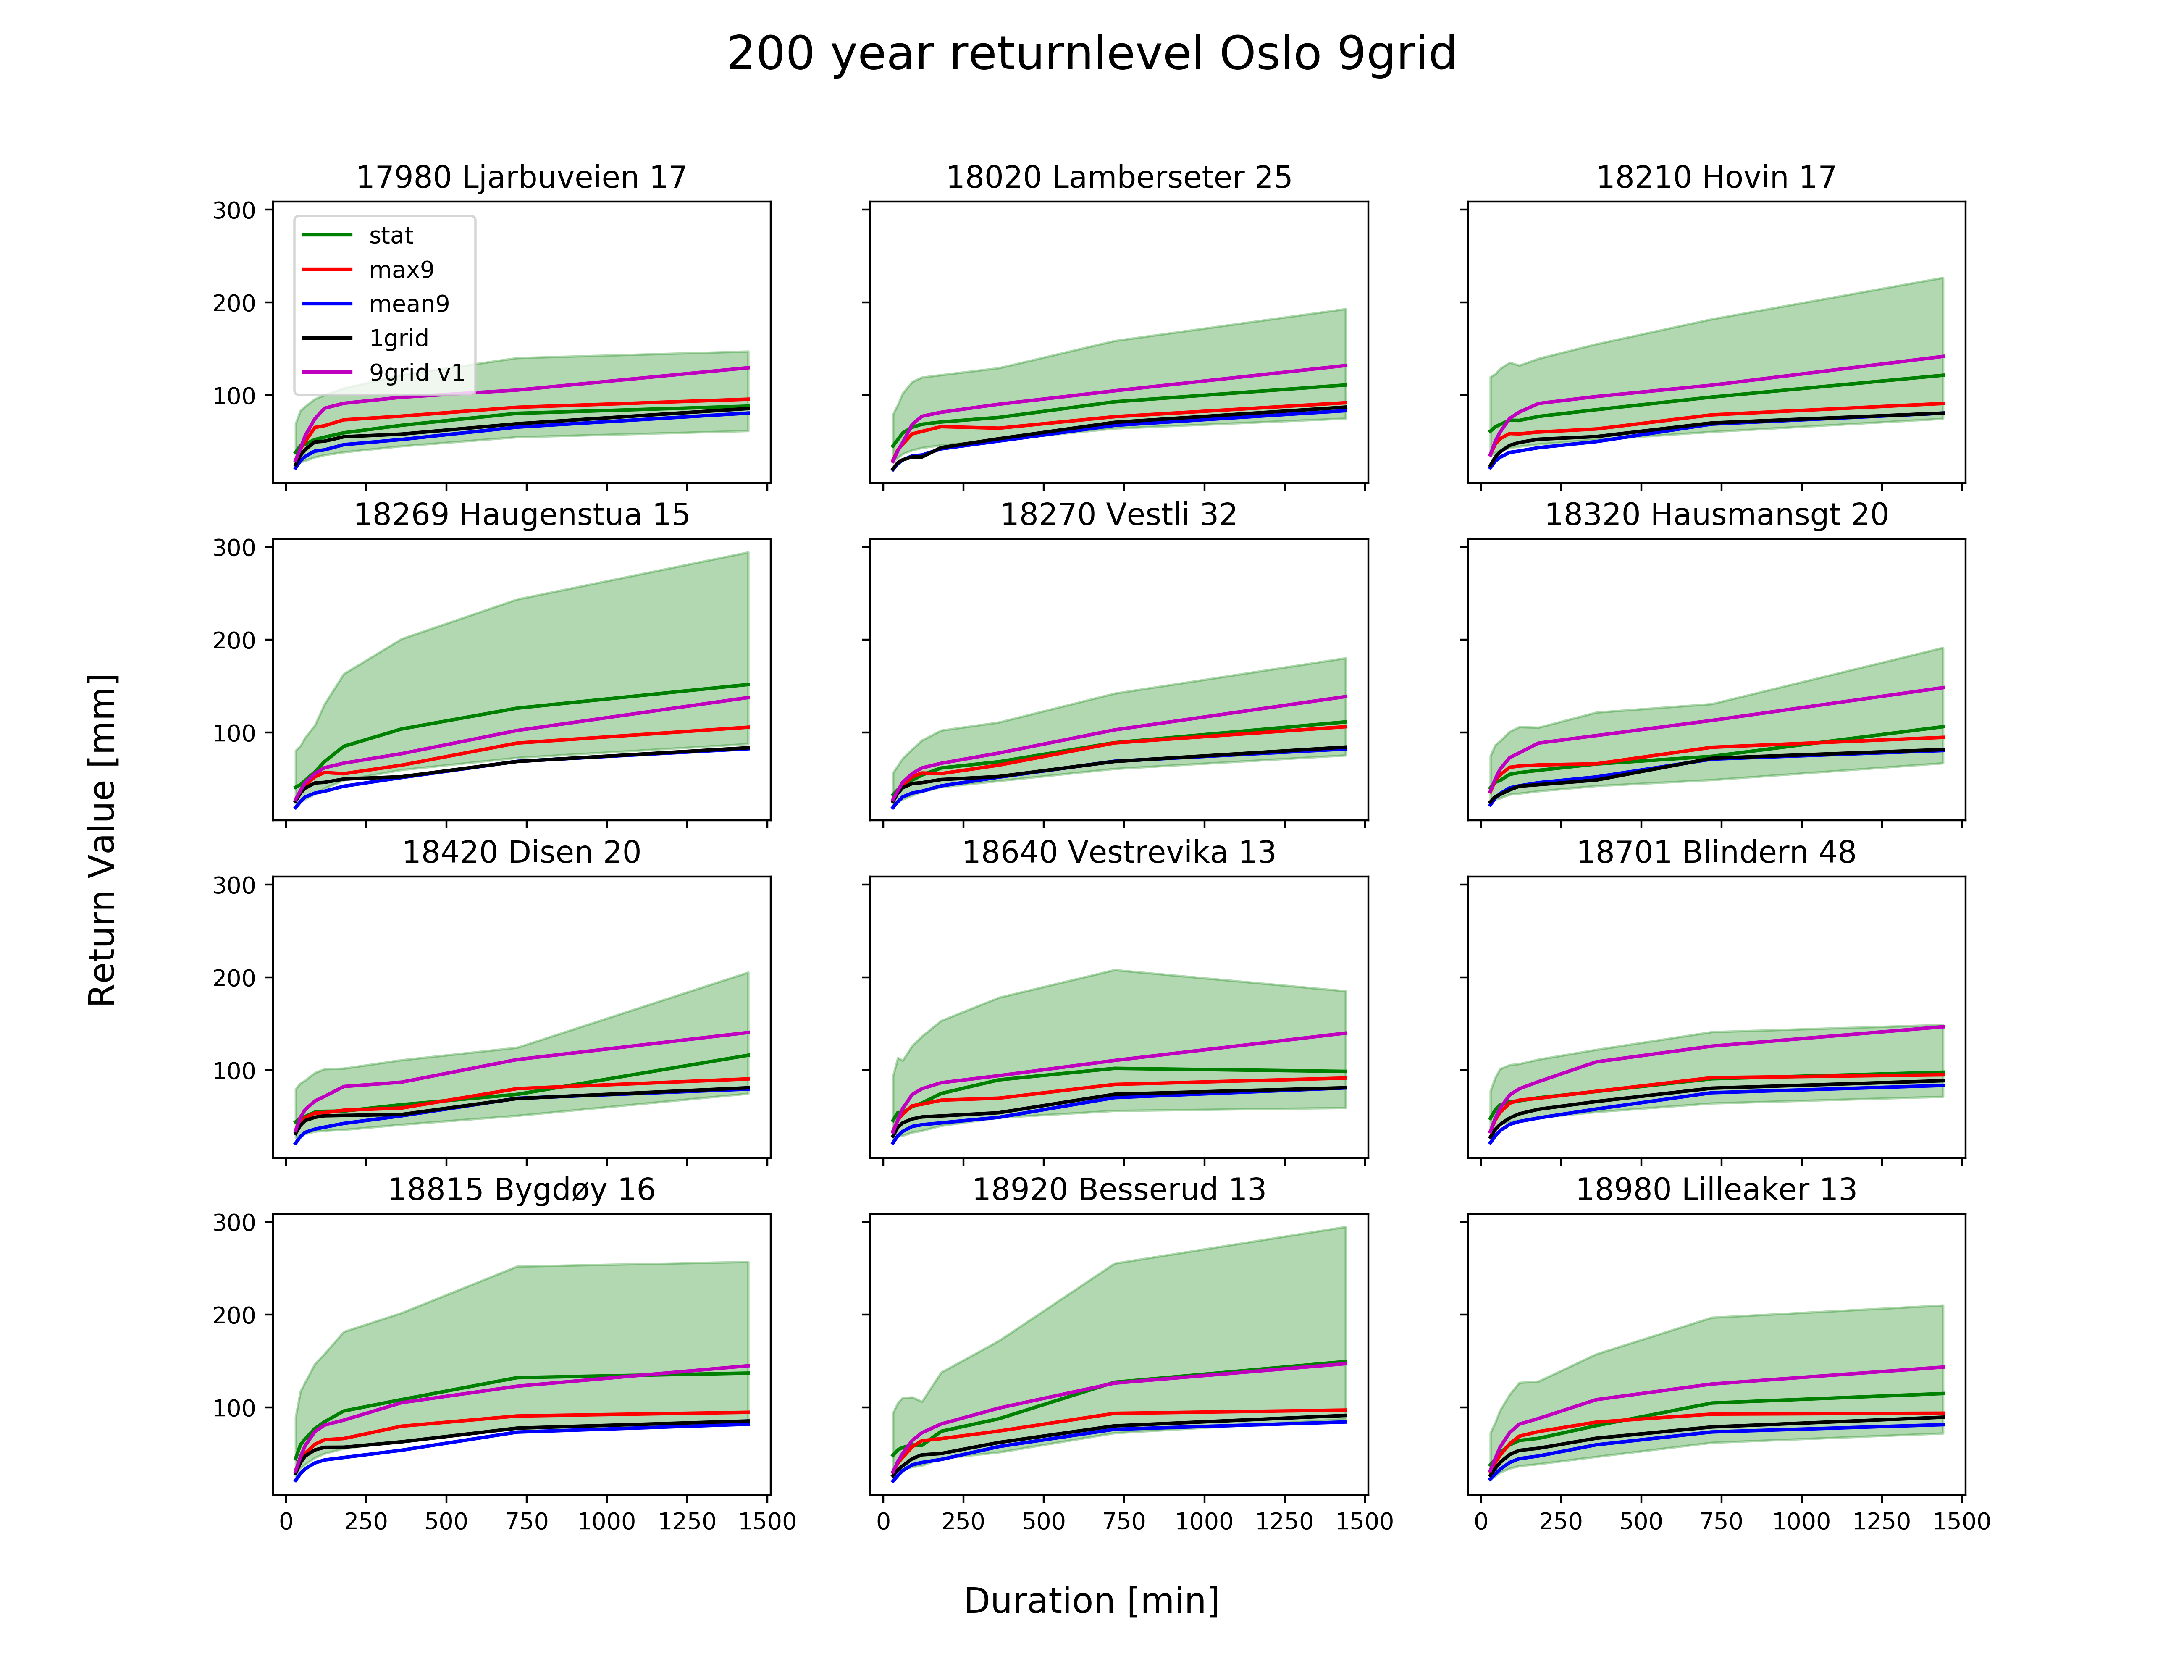
\includegraphics[scale=0.4]{figures/200_retper_ECE_1985_compare.png}
    \caption{Example figure. This is what I am talkin about
    \cite{lind_arome}}
    \label{fig:arome_domain}
\end{figure}

On average for all stations the $MAX$ method overestimate the IDF-values slightly for 2 year returnperiod, and slightly underestimate for all returnperiods larger than 5 years. In table \ref{dist_eval} the realtionship between the respective model and the station-based returnvalues are listed in station- and duration-averaged percentage. For station Haugenstua, Ljabruvegen, Hovin and Besserud it is close to identical to the $STAT$ method for all durations on the 2 year returnperiod. For the larger returnperiods it is the overall method closest to the $STAT$ method, esepecially for the stations with narrow confidence intervals. Providing higher estimates of the returnvalues than the $MEAN$ and the $1GRID$ method but smaller estimates compared to the $9GRID$ the $MAX$ method serves as a middle ground which according to table \ref{dist_eval} is more consistent with the station-based estimates on average for all the Oslo stations. Only for a 200 year returnperiod the station average for the $9GRID$ method is more consistent.        

\begin{table}[hbt!]
\centering
\begin{tabular}{ c c c c c}

Duration & 1grid & 9grid & mean9 & max9 \\
2 & 88.78 & 134.92 & 89.30 & 107.89\\
5 & 82.27 & 125.45 & 79.57 & 100.00\\
10 & 79.29 & 121.10 & 75.09 & 96.37\\
20 & 77.02 & 117.78 & 71.65 & 93.60\\
25 & 76.39 & 116.86 & 70.70 & 92.84\\
50 & 74.66 & 114.33 & 68.07 & 90.73\\
100 & 73.20 & 112.20 & 65.83 & 88.95\\
200 & 71.93 & 110.36 & 63.89 & 87.42
\end{tabular}
\caption{Station- and duration-average returnvalues for each returnperiod in percentage of the station-based station- and duration-average returnvalues. Each column is one method. Values >100 means averge overestimation copared to to the station-based values and values <100 mean underestimation.}
\label{dist_eval}
\end{table}


Even though we (I and Malte) agreed on not using the distance between the curves as any measure, it must be said that the "ax9" method now gives far better overall results compared to the stat.

\subsection{2080-2100}


\begin{thebibliography}{9}

\bibitem{dyrrdal_grid}
Dyrrdal V. Anita, Skaugen Thomas, Stordal Frode, Førland J. Eirik \\
\textit{Estimating areal precipitation in Norway from a gridded dataset}\\
\url{https://doi.org/10.1080/02626667.2014.947289} \\
Hydrological Science Journal, 2015.\\

\bibitem{dyrrdal_bay}
Dyrrdal V. Anita, Lenkoski Alex, Thorarinsdottir L. Thordis, Stordal Frode
\textit{Bayesian hierarchical modeling of extreme hourly precipitation in Norway}
Published: 2014

\bibitem{lapsrate}
@article{article,
author = {Mokhov, I. and Akperov, Mirseid},
year = {2006},
month = {07},
pages = {430-438},
title = {Tropospheric lapse rate and its relation to surface temperature from reanalysis data},
volume = {42},
journal = {Izvestiya, Atmospheric and Oceanic Physics},
doi = {10.1134/S0001433806040037}
}

\bibitem{marshall}
Marshall John, Plumb R. Alan, Atmosphere, ocean and climate dynamics
Book orange blue

\bibitem{lutz_idf}
Lutz Julia, Grinde Lars, Dyrrdal V. Anita
\textit{Estimating Rainfall Design Values for the City of Oslo, Norway - Comparison of Methods and Quantification of Uncertainty}
Published: 2020

\bibitem{seity_arome}
Seity Y, Brousseau P, Malardel S, Hello G, Bénard P, Bouttier F,
Lac C, Masson V (2011) The AROME-France convective-scale
operational model. Mon Weather Rev 139(3):976–991. https ://doi.
org/10.1175/2010M WR342 5.1

\bibitem{rogers}
Rogers R.R, Yau M.K (1996). A Short Course in Cloud Physics. Third Edition.International Series in Natural Philosophy.
Butterworth-Heinemann, Elsevier.
ISBN 0-7506-3215-1

\bibitem{Ahrens}
Essentials of Meteorology, An invitation to the atmosphere.
C. Donald Ahrens

\bibitem{Wallace}
Atmospheric Science, an introductory survey
John M. Wallace, Peter V. Hobbs

\bibitem{Marshall}
Atosphere, Ocean and Climate Dynamics, an introductory text
John Marshall, R. Alan Plumb

\bibitem{lind_arome}
Lind P, Belušić D, Christensen B. O., Dobler A, Kjellström E, Landgren O, Lindstedt D, Matte D, Perdersen A. R, Toivonen E, Wang F
Benefits and added value of convetion-permitting climate modeling over Fenno-Scandinavia.
Published 2020

\bibitem{erai}
Berrisford P, Dee D, Poli P, Brugge R, Fielding K, Fuentes M, Kållberg P, Kobayashi S, Uppala S, Simmons A (2011)
The ERA-Interim archive Version 2.0. ERA Report. ECMWF. Shinfield Park, Reading. URL: https://www.ecmwf.int/node/8174

\bibitem{bengtsson_arome}
Bengtsson L, Andrae U, Aspelien T, Batrak Y et al (2017) The HARMONIE–
AROME model configuration in the ALADIN–HIRLAM
NWP system. Mon Weather Rev 145:1919–1935. https ://
doi.org/10.1175/MWR-D-16-0417.1

\bibitem{belusic_hclim}
Belušić, D., de Vries, H., Dobler, A., Landgren, O., Lind, P., Lindstedt, D., Pedersen, R. A., Sánchez-Perrino, J. C., Toivonen, E., van Ulft, B., Wang, F., Andrae, U., Batrak, Y., Kjellström, E., Lenderink, G., Nikulin, G., Pietikäinen, J.-P., Rodríguez-Camino, E., Samuelsson, P., van Meijgaard, E., and Wu, M.: HCLIM38: a flexible regional climate model applicable for different climate zones from coarse to convection-permitting scales, Geosci. Model Dev., 13, 1311–1333, https://doi.org/10.5194/gmd-13-1311-2020, 2020.

\bibitem{lindstedt_hclim}
Lindstedt D, Lind P, Kjellström E, Jones C (2015) A new regional
climate model operating at the meso-gamma scale: performance
over Europe. Tellus A Dyn Meteorol Oceanogr 67:1. https ://doi.
org/10.3402/tellu sa.v67.24138

\bibitem{lind_hclim}
Lind P, Lindstedt D, Kjellström E, Jones C (2016) Spatial and temporal
characteristics of summer precipitation over central Europe in a
suite of high-resolution climate models. J Clim 29:3501–3518.
https ://doi.org/10.1175/JCLI-D-15-0463.1

\bibitem{gmao}
URL: \url{kilde https://gmao.gsfc.nasa.gov/research/subseasonal/atlas/GEV-RV-html/GEV-RV-description.html}

\bibitem{labus}
Labus, M., Labus, K. Thermal conductivity and diffusivity of fine-grained sedimentary rocks. J Therm Anal Calorim 132, 1669–1676 (2018). \\
URL: \url{https://doi.org/10.1007/s10973-018-7090-5}

\bibitem{muller}
MÜller et al. 2017\\
\textit{AROME-MetCoOp: A Nordic Convective-Scale Operational
Weather Prediction Model}\\
URL: \url{https://doi.org/10.1175/WAF-D-16-0099.1}

\bibitem{metreport}
URL: \url{file:///C:/Users/Eirik%20N/Downloads/Met_info_27_2019_styrtregn_B%C3%A6rum_20190807_v02%20(3).pdf}

\bibitem{finse}
Webpage of Finse Alpine Research Ceenter\\
URL: \url{https://www.finse.uio.no/about/location/}\\
Visited 20th of April 2020

\bibitem{seklima}
Historical precipitation records from Finse.\\
URL: \url{https://seklima.met.no/observations/}

\bibitem{yr}
Webpage of Nowegian forcasting service YR for historical data for Finse.\\
URL: \url{https://www.yr.no/nb/historikk/graf/1-111123/Norge/Vestland/Ulvik/Finse}

\bibitem{hosk}
Hosking, J.R.; Wallis, J.R. Parameter and quantile estimation for the generalized Pareto distribution.
Technometrics 1987, 29, 339–349.
https://www.tandfonline.com/doi/pdf/10.1080/00401706.1987.10488243?needAccess=true

\bibitem{olsson}
Olsson, J.; Södling, J.; Berg, P.;Wern, L.; Eronn, A. Short-duration rainfall extremes in Sweden: A regional
analysis. Hydrol. Res. 2019, 50, 945–960.
https://iwaponline.com/hr/article/50/3/945/65595/Short-duration-rainfall-extremes-in-Sweden-a

\bibitem{huard}
Huard, D.; Mailhot, A.; Duchesne, S. Bayesian estimation of intensity–duration–frequency curves and of
the return period associated to a given rainfall event. Stoch. Environ. Res. Risk Assess. 2010, 24, 337–347.
https://link.springer.com/article/10.1007%2Fs00477-009-0323-1

\bibitem{mohymont}
B. Mohymont, G. R. Demarée, D. N. Faka. Establishment of IDF-curves for precipitation in the
tropical area of Central Africa - comparison of techniques and results. Natural Hazards and Earth
System Science, Copernicus Publications on behalf of the European Geosciences Union, 2004, 4 (3),
pp.375-387. ffhal-00299129f
https://hal.archives-ouvertes.fr/hal-00299129/document

\bibitem{fevd}
URL: https://www.rdocumentation.org/packages/extRemes/versions/2.0-12/topics/fevd
RDocumentation of function: fevd : from the extRemes package in R.

\bibitem{nhat}
(Nhat et al., 2006)
Establishment of Intensity-Duration-Frequency Curves
for Precipitation in the Monsoon Area of Vietnam
Found in local forlder IDF

\bibitem{R}
R Core Team (2013). R: A language and environment for statistical
computing. R Foundation for Statistical Computing, Vienna, Austria.
URL http://www.R-project.org/.

\bibitem{Rextremes}
https://cran.r-project.org/web/packages/extRemes/extRemes.pdf


\end{thebibliography} 

\bibliographystyle{plainnat}

%\bibliography{bib}

\include{appendix}
  
\end{document}